\documentclass[a4paper,12pt]{report}

\usepackage{alltt, fancyvrb, url}
\usepackage{graphicx}
\usepackage{subfigure}
\usepackage{wrapfig}
\usepackage{algorithmic}
\usepackage[utf8]{inputenc}
\usepackage{fontenc}
\usepackage{amsmath,stmaryrd,mathtools,algorithm}
\usepackage{amssymb}
\usepackage{float}
\usepackage{hyperref}
\usepackage{titlesec}

% Remove option to use English naming
\usepackage[italian]{cleveref}

% Questo commentalo se vuoi scrivere in inglese.
\usepackage[italian]{babel}

\title{Relazione per\\``DPG - Dope Party Game''}

\author{Davide Freddi\\Davide Picchiotti\\Miriana Ascenzo\\Riccardo Squarcialupi}
\date{\today}

\begin{document}
 
\maketitle

\tableofcontents

\chapter{Analisi}
\section{Requisiti}
Il software DPG - Dope Party Game consiste in un gioco a turni, in cui l'obiettivo è far arrivare il proprio personaggio in fondo a un tabellone, costituito da uno o più percorsi formati da caselle.
%
Alla fine di ogni turno, vengono fatti fare dei minigiochi a ogni giocatore.

\subsubsection{Requisiti funzionali}
\begin{itemize}
	\item il software deve presentare un menu principale all'avvio, che permetta di avviare il gioco con diverse opzioni, quali numero di giocatori e numero di CPU
	\item il gioco viene giocato da più giocatori nello stesso computer, prendendo il controllo durante il proprio turno
	\item ai giocatori viene fatto tirare un dado, che determina quanti passi vengono fatti all'interno del tabellone
	\item esistono diversi tipi di celle, che possono causare diversi eventi quando un personaggio ci finisce sopra
	\item alla fine di ogni turno viene scelto casualmente un minigioco da far fare a tutti i giocatori, e in base alla posizione nella classifica dei punteggi vengono assegnati dadi migliori o peggiori
	\item ogni CPU ha una difficoltà, che determina i suoi punteggi nei minigiochi
	\item i minigiochi possibili sono:
	\begin{itemize}
	    \item ballgame - bisogna far arrivare una palla in fondo a un percorso il prima possibile, e alcuni muri fanno tornare all'inizio se colpiti
	    \item punchygame - bisogna colpire piu' sacchi possibili, mirando nella direzione giusta
	    \item molegame - bisogna colpire più talpe possibili entro lo scadere del tempo
	    \item jumpgame - bisogna arrivare più in alto possibile rimbalzando su delle piattaforme
	\end{itemize}
\end{itemize}

\section{Analisi e modello del dominio}

Il programma partirà da un menu, che al momento opportuno avvierà il gioco.
%
All'avvio del gioco il menu notificherà il ciclo di gioco (GameCycle), che gestirà una serie di personaggi (Character).
%
I personaggi si muovono all'interno di una griglia (Grid) composta da caselle (Cell), e possono essere controllati o da un giocatore, o da una cpu (CPU), gestita del ciclo di gioco.
%
Alla fine del turno il gamecycle avvierà dei minigiochi (Minigame), che ritorneranno un certo punteggio intero.
%
Le difficoltà primarie potrebbero essere le seguenti:
\begin{itemize}
    \item gestire le cpu in maniera intelligente, evitando di complicare eccessivamente il codice
    \item generare una griglia senza impostarne tutti i dettagli manualmente dal codice
	\item generare diverse configurazioni di griglie con un codice flessibile
	\item individuare una struttura di codice basilare e comune per i minigiochi
    \item gestire le collisioni e la fisica nei minigiochi che lo richiedono
\end{itemize}

\begin{figure}[!t]
\centering{}
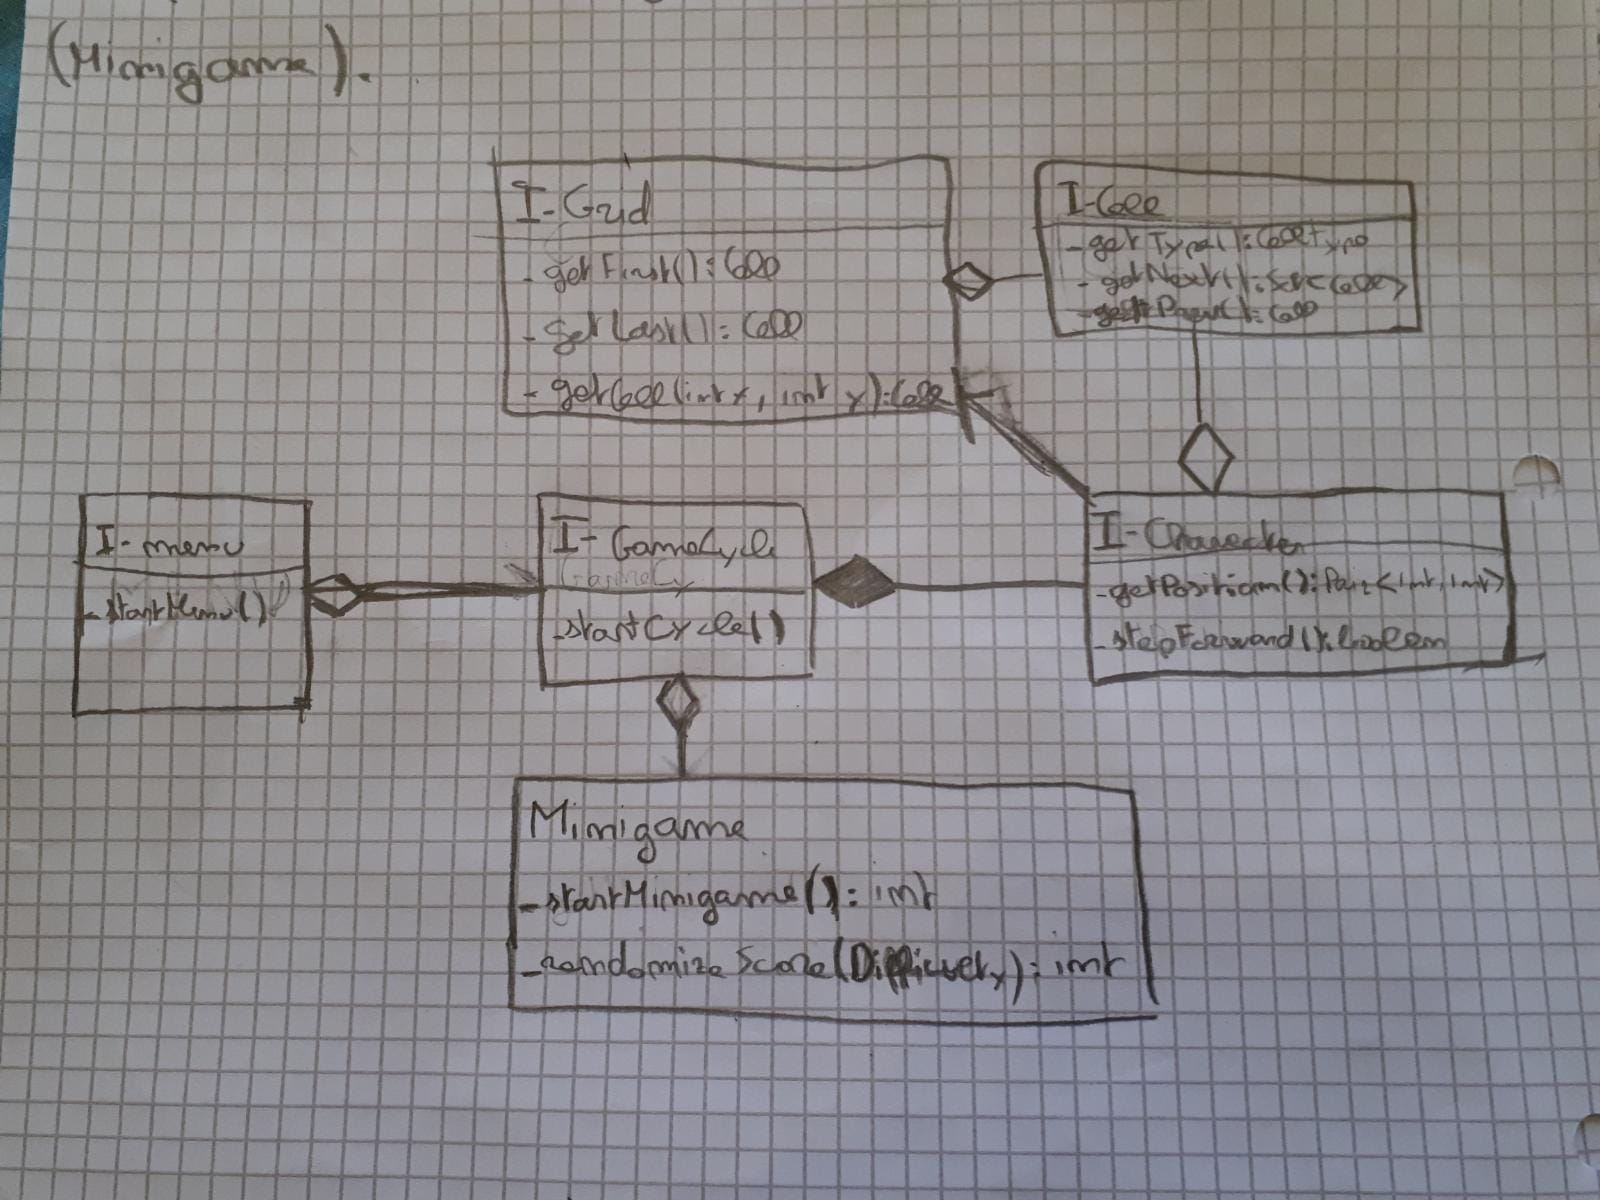
\includegraphics[width=150mm]{images/domain.jpeg}
\caption{Schema UML dell'analisi del problema, con rappresentate le entità principali ed i rapporti fra loro}
\label{img:analysis}
\end{figure}

\chapter{Design}

\section{Architettura}

L'architettura del software segue il pattern architetturale MVC.
%
Il menu è composto da una View (MenuView), e un Controller (MenuController) che ne cattura gli eventi e ne comanda le modifiche.
%
Quando il gioco viene avviato il Controller del menu avvia il ciclo di gioco (GameCycle).
%
Il ciclo di gioco avvia un nuovo thread in background che si occupa di gestire una serie di personaggi e le varie CPU, gestire la sequenza dei turni nel gioco, e aggiornare la View della griglia (Gridview) quando necessario.
%
Il Character rappresenta un personaggio in grado di tirare il proprio dado e spostarsi all'interno della griglia (Grid).
%
La CPU si occupa invece di fare le decisioni che spetterebbero normalmente al giocatore, come scegliere il percorso da fare in un bivio.
%
Il Character tiene traccia della propria posizione tramite un riferimento alla casella (Cell) su cui si trova.
%
La casella contiene delle coordinate e il riferimento alle caselle successive e precedenti nel tabellone.
%
La griglia gestisce le caselle, e permette di ottenere la prima e l'ultima casella del percorso, o una certa casella date delle coordinate.
%
Minigame si occupa di eseuire il minigioco, o ottenere un punteggio per una CPU in base alla sua difficoltà.
%
Ogni minigioco avrà a sua volta delle ulteriori interfacce di View, Controller e Model.

\begin{figure}[!t]
\centering{}
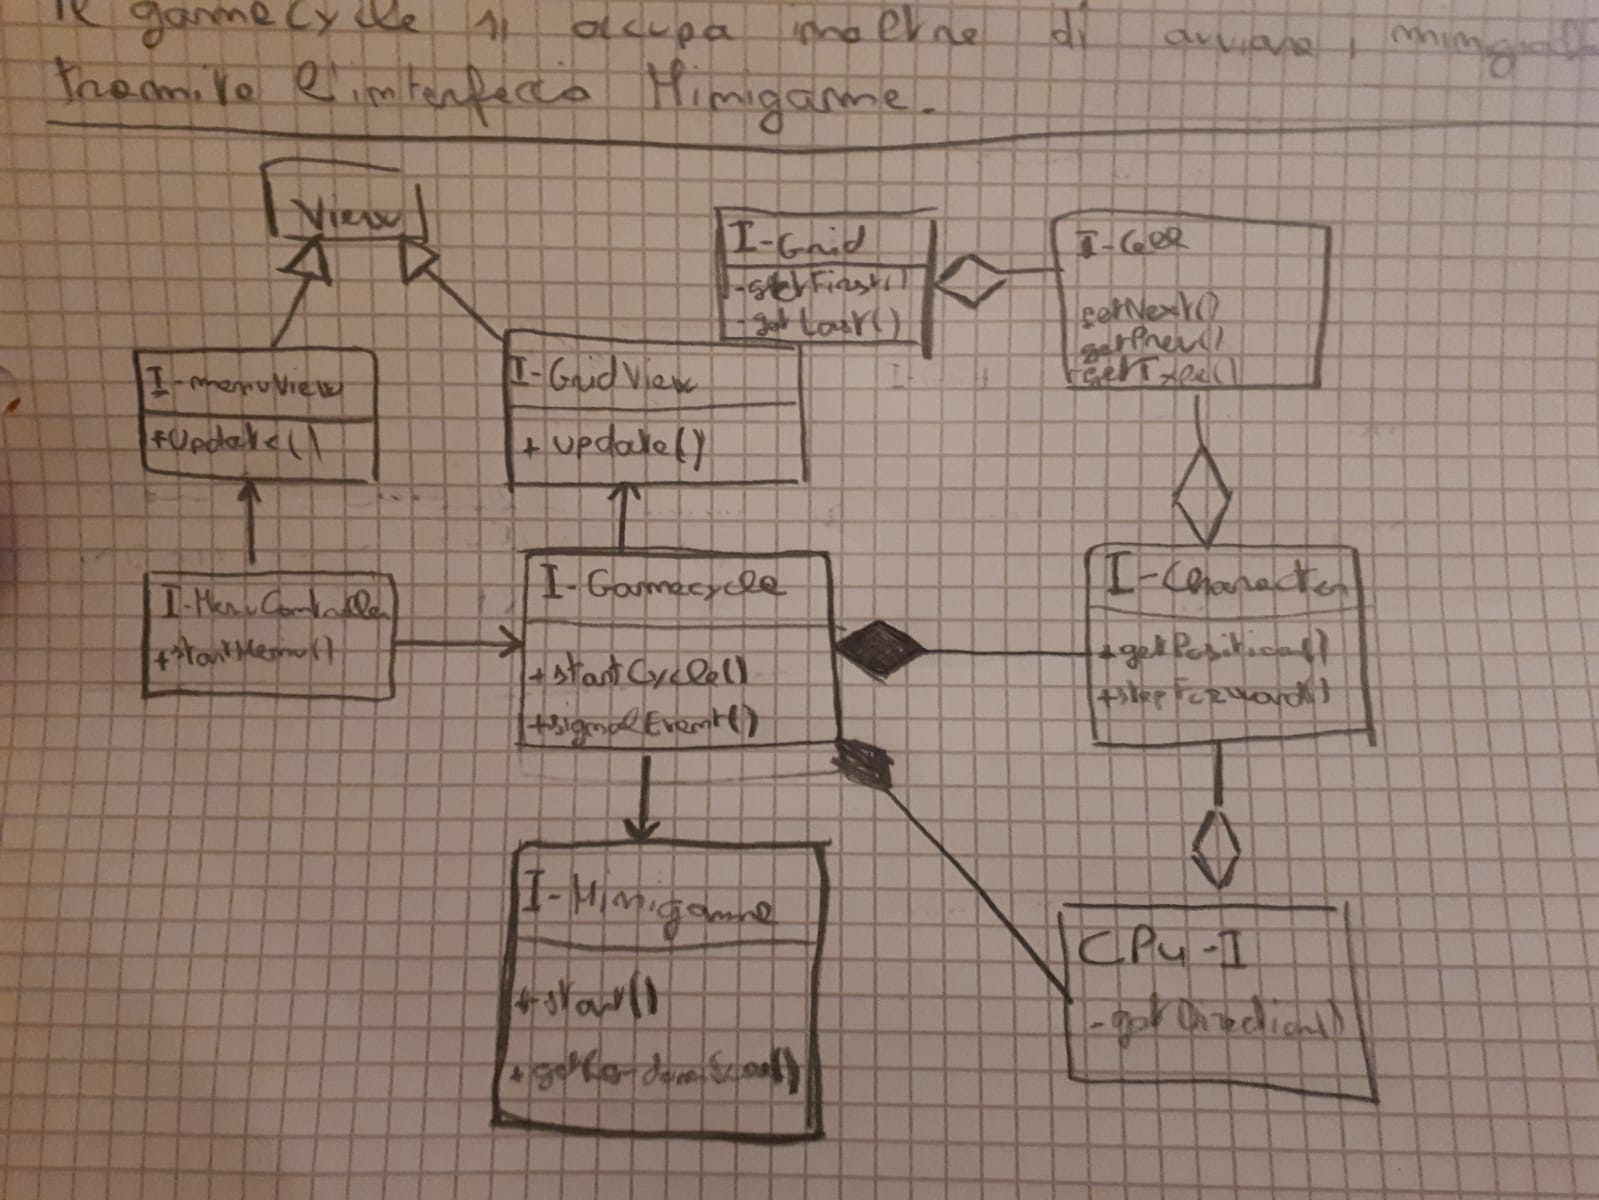
\includegraphics[width=\textwidth]{images/arch.jpeg}
\caption{Schema UML architetturale di DPG. View, GridView e MenuView sono interfacce di view, Gamecycle e Minigame sono interfacce di controller, mentre Grid, Cell e Character sono interfacce di modello.}
\label{img:goodarch}
\end{figure}

\section{Design Dettagliato}

\subsection{Design dettagliato Davide Freddi}
Design dettagliato davide freddi

\subsection{Design dettagliato Davide Picchiotti}
Design dettagliato Davide Picchiotti

\subsection{Design dettagliato Miriana Ascenzo}

A partire dalla classe GridGenerator e dal suo unico metodo generate(), vengono creati prima una Grid (modello del Tabellone di Gioco) composta da più Cell, e poi una GridView (view del Tabellone), che si basa sulla Grid creata.
%
Una Grid viene creata a partire dagli elementi che gli vengono forniti: GridGenerator prende per costruttore una GridType (enum di possibili griglie) e tramite essa cerca nelle resources un file Json corrispondente.
%
In base al Json, genera una griglia diversa usando sempre lo stesso procedimento.
%
La griglia viene dunque generata automaticamente una volta ottenuto il Json che descrive la struttura del Tabellone.
%
La lettura e estrazione dei dati dal file Json avvengono tramite l’uso dei metodi della libreria Jackson.

\begin{figure}[!t]
\centering{}
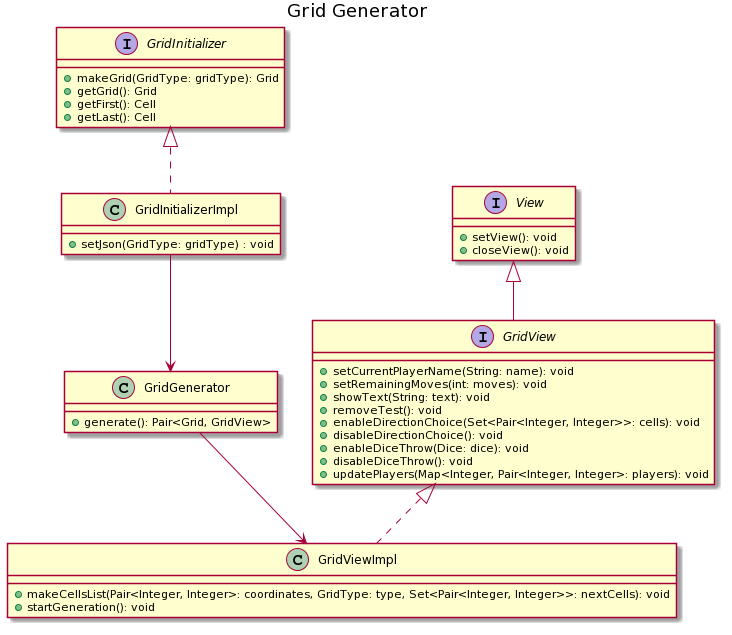
\includegraphics[width=\textwidth]{images/miriana/grid_generator.png}
\caption{Schema UML delle classi di generazione del Tabellone.}
\label{img:gridfactorymethod}
\end{figure}

Gli elementi di GridView che ricevono input dall’esterno, ad esempio i bottoni, hanno il ruolo di informare il gameCycle di quale azione è stata intrapresa da chi sta usando il software.
%
Per fare questo si applica il pattern Observer.
%
Una classe GridObserver ha per Observable GridViewImpl: Se un determinato bottone viene premuto, o una determinata key sulla tastiera viene premuta, viene inviato un segnale al GameCycle.

\begin{figure}[!t]
\centering{}
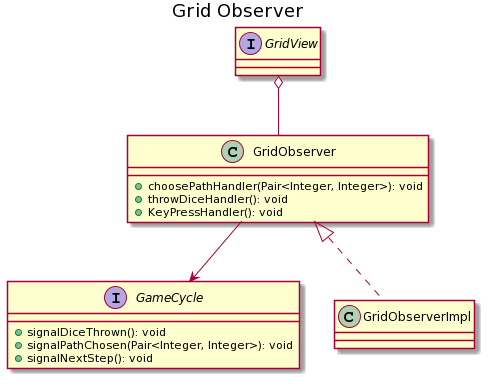
\includegraphics[width=\textwidth]{images/miriana/grid_observer.png}
\caption{Schema UML delle classi di View, e di come interagiscono con il gameCycle. Segue il pattern Observer.}
\label{img:gridobserver}
\end{figure}

I nodi di GridViewImpl vengono aggiornati in runtime ogni volta che gli elementi all’interno del software, quali players, dices, scritte da rappresentare, vengono modificati dal controller (ovvero il gameCycle).
%
per aggiornare i nodi correttamente in runtime, esiste una classe GridViewPlat, che implementa GridView, la quale prende per costruttore una GridViewImpl, creata in GridGenerator, e chiama i suoi metodi nel thread dell’applicazione JavaFX.
%
Questo avviene tramite l’uso di Platform.runLater.
%
Quello che succede in GridGenerator è quindi: una GridViewImpl viene creata a partire da una Grid, e in seguito, a partire da GridViewImpl, viene creata una GridViewPlat, responsabile dell’aggiornamento della View nel thread dell’applicazione JavaFX.
%
Abbiamo un pattern Mediator, per cui gameCycle e GridViewImpl non comunicano direttamente, ma tramite GridViewPlat.

\begin{figure}[!t]
\centering{}
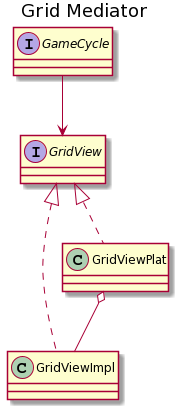
\includegraphics[width=\textwidth]{images/miriana/grid_mediator.png}
\caption{Schema UML di come GameCycle e GridView comunicano. Segue il pattern Mediator.}
\label{img:gridmediator}
\end{figure}

\subsection{Design dettagliato Riccardo Squarcialupi}
Design dettagliato Riccardo Squarcialupi

\chapter{Sviluppo}
\section{Testing automatizzato}

\subsection{Davide Freddi}
\subsection{Davide Picchiotti}
\subsection{Miriana Ascenzo}

È stata sottoposta a test automatici la creazione di una Grid a partire da uno specifico gridType.
%
Vengono fatti dei test sul giusto collegamento fra Celle e sul giusto contenimento o meno di alcune celle nella Grid creata.
%
Per la View sono stati eseguiti dei test automatici facendo uso della libreria TestFX; in particolare sono stati testati il corretto aggiornamento del Label principale nella view (dove appaiono le scritte del tipo “start game”, “dice result”),
%
il corretto aggiornamento della posizione dei player all'interno della mappa, e la possibilità di cliccare o meno il button per tirare il dado in base a se il tiro è abilitato o disabilitato.


\subsection{Riccardo Squarcialupi}

\section{Metodologia di lavoro}

Descrizione separazione?

\subsection{Sezione Davide Freddi}
\subsection{Sezione Davide Picchiotti}
\subsection{Sezione Miriana Ascenzo}

Il ruolo nel gruppo è stato quello di creare strutture dati per le Celle e la Griglia del gioco, la creazione delle stesse a partire da un json, e la creazione di una View che rappresentasse la griglia creata e che si aggiornasse in tempo reale in base ai cambiamenti dettati dal controller.
%
Un problema presentatosi durante la fase d’integrazione, è stato la dimenticanza in fase di design di un metodo “getPrevious” in Cell; il metodo serve per poter implementare la funzionalità “StepBackwards”, ovvero la possibilità di tornare indietro nella griglia.

\subsection{Sezione Riccardo Squarcialupi}


\section{Note di sviluppo}

\subsection{Davide Freddi}
\subsection{Davide Picchiotti}
\subsection{Miriana Ascenzo}

Feature avanzate usate:
\begin{itemize}
    \item lambda
    \item stream
    \item librerie esterne (Jackson, JavaFX, TestFX, Mockito)
\end {itemize}
La libreria Jackson permette di leggere il contenuto di un file json e di tradurlo tramite un mapper e un parser.
%
La classe GridInitializer fa uso di un’altra classe CellParser, con la quale, tramite il mapper, vengono raccolti i dati Cella per Cella e inseriti nella struttura dati.
%
La classe TestFX permette di eseguire test sulla GUI.
%
La classe Mockito permette, in fase di test, di creare classi Mock a partire da interfacce esistenti (simulano il comportamento di classi che implementano tali interfacce).

\subsection{Riccardo Squarcialupi}

\chapter{Commenti finali}

\section{Davide Freddi}
\section{Davide Picchiotti}
\section{Miriana Ascenzo}

Punti di forza:
%
Il lavoro è stato svolto in maniera abbastanza lineare, realizzando in ordine le diverse fasi del progetto.
%
Le classi di generazione del Tabellone di Gioco e di View sono state automatizzate al meglio delle capacità, risultando in una view facilmente sostituibile.
Punti di debolezza:
%
Sono stati fatti errori di distrazione, il che ha richiesto dover tornare indietro nel codice più volte pe trovare tali errori e correggerli.


\section{Riccardo Squarcialupi}

\appendix
\chapter{Guida utente}

Spiegazione comandi e utilizzo del gioco

All'avvio del gioco compare un menù: premere start avvia un game in impostazioni standard (2 giocatori, di cui uno è una CPU).
%
Se si vuole modificare il numero di giocatori e/o il numero di CPU, premere Options ed inserire le preferenze.
%
Una volta premuto start il game inizia con i giocatori sulla casella start.
%
Da qui bisogna seguire le istruzioni che vengono dettate nel riquadro bianco più in alto:
\begin {itemize}
	\item quando appare l'istruzione "continue..", premere invio per proseguire
	\item quando appare l'istruzione "Throw the Dice!", il bottone dado sottostante verrà abilitato: premere il bottone per tirare il dado
	\item quando appare l'istruzione "choose the direction on the map", due bottoni verrano abilitati: premere il bottone corrispondente alla casella che si vuole raggiungere
\end {itemize}
Ogni turno finisce con un minigioco: ottenere più punti possibili per vincere dadi migliori da tirare.
Istruzioni minigiochi:
\begin {itemize}
	\item ballgame: premere le frecce direzionali per comandare la palla rossa. Raggiungere il traguardo evitando i muri rossi nel tempo limite(punteggio basato sul tempo impiegato).
	\item punchygame: premere le frecce direzioni destra e sinistra per colpire i sacchi da boxe rossi. Colpirne il maggior numero nel tempo limite (punteggio basato sul numero di sacchi colpiti).
	\item jumpgame: premere le frecce direzionali per comandare il quadratino. Saltare più piattaforme possibili senza cadere o toccare i bordi laterali della finestra (punteggio basato sul numero di piattaforme saltate).
	\item molegame: premere start per avviare il minigioco: cliccare su più talpe possibili nel tempo limite (punteggio basato sul numero di talpe cliccate).
\end {itemize}
Il gioco finisce quando un giocatore raggiunge l'ultima casella del Tabellone, vincendo il game.


\bibliographystyle{abbrv}
\bibliography{template}

\end{document}
